% !TeX program = xelatex
% Standalone source: all figures and bibliography are embedded.
\documentclass[UTF8,11pt,a4paper,fontset=fandol]{ctexart}
\usepackage[left=2.25cm,right=2.25cm,top=2.25cm,bottom=2.3cm]{geometry}
\usepackage{amsmath,amssymb,bm}
\usepackage{graphicx,booktabs,tabularx,longtable,array,multirow}
\usepackage{caption,float,placeins}
\usepackage{xcolor,tikz,pgfplots}
\usetikzlibrary{arrows.meta,positioning,calc,fit}
\pgfplotsset{compat=1.18}
\IfFileExists{hycolor.sty}{%
  \usepackage[unicode,colorlinks=true,linkcolor=blue!45!black,citecolor=green!35!black,urlcolor=blue!45!black]{hyperref}
}{\usepackage{url}}
\usepackage{xurl}
\newcolumntype{Y}{>{\raggedright\arraybackslash}X}
\newcolumntype{P}[1]{>{\raggedright\arraybackslash}p{#1}}
\newcommand{\ap}{\mathrm{AP}}
\newcommand{\LN}{\operatorname{LN}}
\newcommand{\sigmoid}{\operatorname{sigmoid}}
\newcommand{\softplus}{\operatorname{softplus}}
\newcommand{\GELU}{\operatorname{GELU}}
\newcommand{\SiLU}{\operatorname{SiLU}}
\newcommand{\diag}{\operatorname{diag}}
\newcommand{\R}{\mathbb{R}}
\newcommand{\pp}{\,\mathrm{pp}}
\newcommand{\sourceNote}[1]{\par\smallskip{\footnotesize #1}\par}
\setlength{\parskip}{0.22em}
\setlength{\parindent}{2em}
\setlength{\emergencystretch}{2em}
\renewcommand{\arraystretch}{1.18}
\setlength{\leftmargini}{2em}
\captionsetup{font=small,labelfont=bf}
\tikzset{box/.style={draw=blue!40!black,rounded corners=2pt,fill=blue!4,align=center,font=\small,minimum height=9mm,inner sep=5pt}, arrow/.style={-{Latex[length=2mm]},thick,draw=black!65}, ctrl/.style={arrow,dashed,draw=orange!75!black}}
\title{面向 SAR 图像的可靠性引导 Mamba 状态传播方法\\[0.5em]
\large Reliability-Guided Selective State Propagation in Mamba for SAR Imagery}
\author{}
\date{中文修订稿 \quad 2026 年 10 月 5 日}
\begin{document}
\maketitle

\begin{abstract}
合成孔径雷达（SAR）图像中的目标散射中心、背景杂波与散斑起伏可以产生相近的局部响应幅值，因而仅凭响应强度难以判断信息对结构表征的价值。针对这一问题，本文提出可靠性引导的选择性状态传播机制（RGSP），以局部趋势和邻域变化作为可靠性建模的结构线索，在 Mamba 已有输入选择性的基础上调节状态更新。该机制首先在中间特征空间执行可学习局部残差修正，随后通过感知特征重要性模块（PFIM）学习空间控制量，并将其注入选择性扫描的输入驱动与离散化步长。本文给出与实现一致的递推形式，区分当前输入写入、历史状态衰减和输出门控的作用。在 SSDD 五变体、三随机种子的已有测试记录中，完整 RGSP 的 $\ap_{50:95}$ 为 $42.91\pm1.13\%$，基线为 $42.03\pm3.47\%$；DS-only 和 PFIM-only 分别为 $43.98\pm1.44\%$ 和 $43.12\pm1.70\%$。完整组合未超过 DS-only，逐位置重要性也未超过图像级对照。分类、语义分割和变化检测的探索记录进一步显示结果对任务及接入方式的依赖。上述结果揭示了局部结构处理、调制位置与空间粒度之间的非简单叠加关系，为 SAR 状态空间模型的设计提供了可复现的机制描述与实证分析。
\end{abstract}
\noindent\textbf{关键词：}合成孔径雷达；Mamba；选择性状态空间模型；局部结构；状态传播；空间重要性

\section{引言}\label{sec:intro}
合成孔径雷达（Synthetic Aperture Radar，SAR）具有全天时、全天候成像能力，已用于海面舰船监测、机场目标识别和地表变化分析。公开舰船基准揭示了近岸背景、小目标和密集停泊等场景对识别与定位的挑战\cite{ssdd2021}；SAR-AIRcraft-1.0 则体现了飞机散射点离散、尺度差异和机场强干扰带来的困难\cite{saraircraft2023}。不同于自然光学成像，SAR 局部响应受目标散射特性、成像几何和相干成像过程共同影响。较强响应既可能对应有意义的目标散射中心，也可能来自背景杂波；弱响应同样可能携带细小目标或边界信息。因此，响应强度与任务相关结构价值并不等价。有效的 SAR 表征不仅需要较大范围的上下文，还需要利用局部结构判断信息应以何种方式参与后续特征更新。

卷积网络通过层级结构聚合局部信息，残差学习使深层视觉表示的优化成为可能\cite{resnet2015}。视觉 Transformer 则通过图像块之间的自注意力建立远距离联系\cite{vit2020}，其中全局注意力的成对交互在高分辨率特征上带来较高的存储与计算成本。Mamba 利用输入依赖的选择性状态空间模型（Selective State Space Model，SSM）控制信息写入与状态演化，其选择性扫描在固定通道数和状态维数时具有随序列长度线性增长的计算复杂度\cite{mamba2023}。Vision Mamba（Vim）通过双向状态空间建模扩展视觉序列表征\cite{vim2024}；VMamba 通过二维选择性扫描（SS2D）组织四条空间扫描路线\cite{vmamba2024}。进一步地，Mamba YOLO 将状态空间建模与层级目标检测结构结合\cite{mambayolo2024}，为研究 SAR 特征在局部细节与长程关联之间的传播方式提供了合适接口。

Mamba 已经具有内容选择能力，但其输入依赖参数并不天然等价于对 SAR 结构可靠性的显式建模。本文所讨论的可靠性，是局部响应在给定任务及标签保持扰动下持续提供有用结构信息的可依赖程度；它既不是像素幅度，也不等同于前景概率。局部趋势与邻域变化可为这一性质提供线索，却不能单独判定可靠性：离散强散射点可能属于目标，高局部变化也可能对应重要边缘。由此，本文研究的问题不是替代 Mamba 已有的选择性，而是：\emph{能否显式引入 SAR 局部结构线索，进一步调节当前响应的状态写入及后续状态演化？}

已有遥感 Mamba 研究从不同方面增强空间表征。RS-Mamba 面向大幅面遥感图像研究密集预测\cite{rsmamba2024}，RSMTMamba 研究跨任务特征学习\cite{rstmtmamba2025}，MaDiNet 将 Mamba 引入 SAR 目标检测框架\cite{madinet2025}。在这些研究基础上，本文聚焦局部结构线索进入选择性递推的具体位置：扫描输入驱动决定当前信息以何种幅度写入状态，离散化步长则同时参与历史状态衰减和当前输入写入。这一设计位置不同于仅在扫描输出端乘以空间权重，也不要求把所有局部起伏都解释成噪声。

基于上述观察，本文提出可靠性引导的选择性状态传播机制（Reliability-Guided Selective State Propagation，RGSP），其核心包括局部响应修正、空间重要性估计和状态调制。首先，在中间特征上沿扫描序列估计可学习局部趋势，并利用相对趋势的残差修正扫描前响应。随后，感知特征重要性模块（Perceptual Feature Importance Module，PFIM）结合趋势特征与二维邻域变化，学习用于状态调制的空间重要性。所得控制量进一步作用于输入驱动与离散化步长，使局部结构线索直接参与选择性递推。这里的可靠性是结构线索选择的设计目标，实际学习量是由下游任务损失优化的重要性；本文不将二者预设为同一可测量变量，也不以恢复去斑图像为目标。

本文以 SAR 目标检测为主要验证场景，分析 SSDD 上五种变体、三个随机种子的完整记录，并结合分类、分割与变化检测的探索性结果讨论适用范围。实验组织分别回答整体替换设计、模块组合以及空间粒度三个问题，不以不同协议下的公开数值替代内部对照。现有完整组合未显示对 DS-only 的优势，这使局部修正与重要性调制之间的协同关系成为需要独立检验的设计问题，而非由模块叠加即可得到的结论。

\begin{figure}[tbp]
\centering
\begin{tikzpicture}[node distance=6mm]
\node[box,text width=3.2cm] (sar) at (0,0) {SAR 局部响应\\强度不等于结构价值};
\node[box,text width=3.2cm] (context) at (4.9,0) {可学习结构描述\\局部趋势与邻域变化};
\node[box,text width=3.2cm] (state) at (9.8,0) {选择性状态更新\\输入驱动与离散化步长};
\draw[arrow] (sar)--(context);
\draw[arrow] (context)--(state);
\node[align=center,font=\small,text width=14cm] at (4.9,-1.35)
{研究假设：显式局部结构线索能否补充 Mamba 已有的输入选择性？\\验证层次：整体变体比较、同结构机制控制、跨任务适用边界。};
\end{tikzpicture}
\caption{研究动机与验证问题。图为概念示意，不是从图像真值测得的可靠性图；PFIM 输出的空间重要性与实际可靠性的对应关系需独立检验。}
\label{fig:motivation}
\end{figure}

本文的主要贡献如下：
\begin{enumerate}
\item 提出面向 SAR 特征的 RGSP 状态传播设计，将局部结构线索与选择性递推相联系，明确输入驱动和离散化步长两类调制位置。
\item 设计可学习局部残差修正与 PFIM 空间重要性模块，给出完整张量定义、初始化和递推实现，并分析其与输出重加权及原始视觉状态空间块的区别。
\item 基于 SSDD 多种子变体比较，分析单模块、完整组合及重要性空间粒度的表现；结合跨任务记录，讨论接入方式、训练条件和结构细节对适用范围的影响。
\end{enumerate}

\section{相关工作}\label{sec:related}
\subsection{SAR 局部统计、图像去斑与任务表征}
局部统计长期用于图像增强和噪声滤波。Lee 滤波利用局部统计构造自适应图像估计，为局部响应与邻域背景之间的关系提供了经典建模思路\cite{lee1980}。Speckle-Free SAR Image Ship Detection 则直接研究散斑处理与舰船检测的联系\cite{specklefree2021}。这些工作提示，局部响应处理应结合下游任务理解：图像域的平滑程度、视觉质量和目标定位精度不是同一个优化目标。

近期状态空间模型也被用于 SAR 图像复原。RSS-Net 面向 SAR 图像去噪构建 Mamba 网络\cite{rssnet2026}；MambaDIP 将 Mamba 用于深度图像先验框架下的去斑与增强\cite{mambadip2026}。RGSP 与这些方法的区别在于处理对象和优化位置：本文在中间特征域修正局部残差，并进一步控制递推输入与步长，没有独立的干净图像重建输出或复原损失。二维邻域标准差在本文中是特征描述子，而非估计真实散斑方差的物理模型。

\subsection{视觉与遥感选择性状态空间模型}
Mamba 通过输入相关的 $\Delta$、$B$、$C$ 参数实现内容选择和长程序列建模\cite{mamba2023}。因此，“选择哪些信息传播”本身不是本文新引入的问题。Vim 的双向建模\cite{vim2024}和 VMamba 的四路线 SS2D\cite{vmamba2024}分别处理视觉序列的方向性与二维空间组织。Mamba YOLO 在检测网络中结合状态空间建模和局部特征处理\cite{mambayolo2024}，构成本研究检测实现的直接架构背景。

在遥感应用中，RS-Mamba 研究大幅面图像的密集表征\cite{rsmamba2024}，RSMTMamba 研究跨任务信息学习\cite{rstmtmamba2025}。这类研究与本文的关系是互补的：空间序列组织决定上下文如何被访问，局部结构条件化调制决定访问到的信息如何参与递推。当前 RGSP 实现采用单向扫描块替换原始四向块，两种因素在整体检测对照中同时变化；第\ref{sec:integration}节明确披露这一实现差异。

\subsection{SAR-Mamba 与特征重加权}
MaDiNet 是与本文直接相关的 SAR 检测研究，其正式版本发表于 TCSVT\cite{madinet2025}。可核对的预印本具体描述了 MambaSAR、多方向 SAR-SSM 以及局部与全局分支的结合\cite{madinet2024v1}。本文以这些可定位的设计为比较对象，不将版本间不同的文字、模型代码和数值混合为同一冻结实现。MCMN 则将 Doppler 与散射感知特征和 Mamba-CNN 多尺度网络相结合，研究 PolSAR 舰船检测\cite{mcmn2026}。已有工作已经从输入特征、扫描结构和任务框架等层次利用 SAR 信息，本文的定位因而不能建立在“首次把 Mamba 用于 SAR”之上。

特征重加权提供了另一类直接相关的设计。CBAM 在通道和空间维度学习注意力，并对特征进行乘性细化\cite{cbam2018}。RGSP 的输入驱动调制同样包含乘性权重，但其步长分支直接参与递推系数的形成。另一方面，若将普通注意力放在 $\Delta,B,C$ 的生成之前，它也会间接改变状态更新；因此，区分二者应依赖相同结构、相同容量和不同注入位置的对照，而非仅凭“内部调制”这一名称。

\begin{table}[!htbp]\centering\small
\caption{代表性设计的作用位置。表中区分设计接口，不据此推断性能优劣。}
\label{tab:related}
\begin{tabularx}{\linewidth}{P{2.5cm}P{3.25cm}Y}
\toprule
设计 & 主要作用位置 & 与本研究的联系\\
\midrule
局部统计滤波\cite{lee1980} & 图像域局部估计 & 提供局部统计背景；与任务驱动特征变换不同\\
VMamba\cite{vmamba2024} & 二维扫描组织 & 四向空间递推；是原始 VSS/SS2D 的直接背景\\
MaDiNet 预印本\cite{madinet2024v1} & 检测框架与 MambaSAR & 结合扫描和多分支表征；版本需单独识别\\
MCMN\cite{mcmn2026} & 输入线索与混合多尺度网络 & 使用 Doppler/散射特征；输入模态与本文不同\\
CBAM\cite{cbam2018} & 通道和空间特征细化 & 是注入位置对照的代表，而非自动等价于输出注意力\\
RGSP & 局部特征修正、扫描驱动与步长 & 研究结构描述子参与选择性递推的具体方式\\
\bottomrule
\end{tabularx}
\end{table}
\FloatBarrier

\section{方法}\label{sec:method}
\subsection{问题定义与选择性递推}
设输入特征为 $F\in\R^{b\times d\times H\times W}$，其中 $b$ 为批大小、$d$ 为通道数。将空间维按行优先顺序展平，序列长度为 $L=HW$。当前实现先进行逐 token 的通道 LayerNorm：
\begin{equation}
X=\LN\!\left(\operatorname{Flatten}_{HW}(F)\right)\in\R^{b\times L\times d}.
\label{eq:tokens}
\end{equation}
本文用 $m$ 表示状态维数，避免与序列长度混淆。选择性 SSM 根据当前内容生成输入依赖参数，沿序列更新隐藏状态\cite{mamba2023}。在本文采用的扫描实现中，通道 $c$、状态维 $n$ 上的递推为
\begin{equation}
h_{t,c,n}=\exp(\Delta_{t,c}A_{c,n})h_{t-1,c,n}
          +\Delta_{t,c}B_{t,n}u^{\mathrm{scan}}_{t,c},
\qquad h_{0,c,n}=0.
\label{eq:recurrence}
\end{equation}
其中 $A\in\R^{d\times m}$，$B_t,C_t\in\R^m$，$\Delta_t\in\R^d_{>0}$。$B_t,C_t$ 在通道间共享其状态向量，$\Delta_t$ 具有通道相关性。式\eqref{eq:recurrence}采用实现中的 $\Delta B u$ 输入写入形式，而非未经说明地替换为连续系统精确零阶保持离散化的输入项。

RGSP 将局部结构线索引入这一递推的两个位置：一是构造并缩放 $u^{\mathrm{scan}}_t$，二是修正 $\Delta_t$ 的生成。这里没有新增独立的历史状态乘性门；历史状态的衰减通过 $\exp(\Delta A)$ 实现。

\subsection{局部响应修正}
对归一化序列执行核宽为 $k=3$ 的逐通道一维卷积，定义局部趋势、趋势残差和修正特征：
\begin{align}
\bar X&=\operatorname{DWConv1D}_{k=3}(X),\\
R&=X-\bar X,\qquad \widetilde X=X-\lambda_sR.
\label{eq:correction}
\end{align}
卷积权重以 $1/3$ 初始化，随后参与训练；$\lambda_s$ 是块级可学习标量。当前检测块以 $\lambda_s=0.5$ 初始化，不是独立类构造函数中未被该调用路径使用的默认值。式\eqref{eq:correction}旨在通过任务训练调整响应相对局部趋势的偏离，而不预先把残差全部判为噪声。

这一操作有两个重要边界。首先，卷积沿展平序列计算，行末与下一行行首会成为序列邻居，因而不是二维 $3\times3$ 滤波。其次，卷积核和 $\lambda_s$ 均未施加保证平滑性的约束。只有在额外满足 $\lambda_s\in[0,1]$ 且趋势算子具有平滑性质时，$\widetilde X=(1-\lambda_s)X+\lambda_s\bar X$ 才能解释为向趋势的凸组合收缩；本文不把这一附加性质当作现实现的保证。

\subsection{PFIM：结构条件化空间重要性}
将 $\widetilde X$ 恢复为二维特征，对每个通道计算 $3\times3$ 邻域标准差：
\begin{equation}
S=\sqrt{\max\!\left(\mathcal P(\widetilde X^{\,2})-
                    \mathcal P(\widetilde X)^{2},\,0\right)+\epsilon},
\qquad \epsilon=10^{-5},
\label{eq:std}
\end{equation}
其中 $\mathcal P$ 为局部均值池化，图像边界不将填充值计入有效样本。再展平 $S$，以趋势和局部变化构造描述子：
\begin{equation}
V_t=[\bar X_t,S_t],\qquad
I_t=\sigmoid\!\left(W_2\GELU(W_1\LN(V_t)+b_1)+b_2\right).
\label{eq:pfim}
\end{equation}
隐藏宽度为 $d_h=\max(\lfloor d/4\rfloor,16)$。PFIM 输出 $I\in(0,1)^{b\times L\times1}$，即每个位置一个标量，而非每通道一个独立权重；后续运算沿通道和状态维广播。最后一层权重、偏置零初始化，故初始 $I_t=0.5$。

PFIM 仅通过下游任务损失联合训练，没有独立可靠性标签或概率校准目标。低标准差不必对应高重要性，高标准差也不必对应低重要性；两者的关系由任务训练决定。本文因此将 $I_t$ 精确定义为\emph{结构条件化的空间控制量}。可靠性解释是否成立，需要检验它与独立定义的结构稳定性和任务有效性之间的关系，而不是用 $I_t$ 自身定义可靠性后再自证。

图像级对照在局部预测之后求平均：
\begin{equation}
I^{\mathrm{global}}=\frac{1}{L}\sum_{t=1}^{L}I_t,\qquad
I^{\mathrm{global}}_t=I^{\mathrm{global}}.
\label{eq:global}
\end{equation}
这与“先对描述子求平均再经过非线性预测”不同。它只去除 PFIM 控制量的位置差异，并不去除内容流、能量项和基础步长的位置变化。

\subsection{输入驱动与离散化步长调制}\label{sec:modulation}
修正特征先经无偏置线性层分为内容分支和输出门控分支：
\begin{equation}
[u_t,z_t]=W_{\mathrm{in}}\widetilde X_t,\quad
B_t=W_Bu_t,\quad C_t=W_Cu_t,\quad A=-\exp(A_{\log}).
\label{eq:projection}
\end{equation}
因此，$B_t,C_t$ 来自尚未乘输入驱动权重的 $u_t$，不能把它们改写为由 $u^{\mathrm{scan}}_t$ 生成。局部修正则通过改变 $\widetilde X_t$ 间接影响这些分支。

\paragraph{输入驱动。}
定义逐位置趋势能量
\begin{equation}
E_t=\frac{\|\bar X_t\|_2}{\sqrt d}.
\end{equation}
能量条件因子与重要性因子分别为
\begin{align}
\gamma_t&=g_{\min}+(1-g_{\min})
 \sigmoid\!\left(-\alpha s_nE_t+\beta_i(I_t-0.5)\right),\\
w_t&=\max\!\left(0.1,1+\tanh(\rho_i)(I_t-0.5)\right),\\
q_t&=\gamma_tw_t,\qquad u^{\mathrm{scan}}_t=q_tu_t .
\label{eq:drive}
\end{align}
其中 $g_{\min}=0.5$，$s_n=0.1$ 为固定系数，不是从图像估计的物理噪声标准差。$\gamma_t$ 与 $w_t$ 共同作用于同一个当前输入驱动位置，不分别对应“历史保留门”和“当前写入门”。$g_{\min}$ 是输入缩放因子的下界参数，不是隐藏状态保留率下界。

\paragraph{离散化步长。}
PFIM 在基础步长的 logits 上加入控制项：
\begin{equation}
\Delta_t=\softplus(W_\Delta u_t+b_\Delta+\eta_i I_t).
\label{eq:delta}
\end{equation}
softplus 在扫描核之外执行一次，保证 $\Delta_t>0$。$\alpha,\beta_i,\rho_i,\eta_i$ 均为可学习标量，初始化分别为 $0.5,1,1,0.1$，训练中不约束符号。因此，当前实现不保证更高 $I_t$ 在各分支上都产生更强写入或更长保留。

\paragraph{输出。}
递推后的状态由 $C_t$ 读出，再加修正特征的通道旁路：
\begin{equation}
y_{t,c}=\sum_{n=1}^{m}C_{t,n}h_{t,c,n}+D_c\widetilde X_{t,c},
\qquad o_t=W_{\mathrm{out}}\bigl(y_t\odot\SiLU(z_t)\bigr).
\label{eq:output}
\end{equation}
当前扫描核接收 \texttt{D=None}、\texttt{z=None} 和 \texttt{delta\_softplus=False}，对应旁路和门控均在核外实现。式\eqref{eq:output}中的旁路输入是 $\widetilde X$，不是 $q u$。

\begin{figure}[tbp]\centering
\begin{tikzpicture}[scale=.96,transform shape,
every node/.append style={font=\footnotesize}]
\node[box,text width=1.75cm] (x) at (0,0) {归一化序列\\$X$};
\node[box,text width=1.75cm] (corr) at (2.7,0) {局部修正\\$\widetilde X$};
\node[box,text width=1.75cm] (proj) at (5.4,0) {内容投影\\$u,z,B,C$};
\node[box,text width=1.75cm] (drive) at (8.1,0) {驱动调制\\$u^{\rm scan}=q u$};
\node[box,text width=1.75cm] (scan) at (10.8,0) {状态递推\\$h_t$};
\node[box,text width=1.75cm] (out) at (13.5,0) {读出门控\\$o_t$};
\node[box,text width=1.75cm] (trend) at (2.7,1.85) {序列趋势\\$\bar X$};
\node[box,text width=2.3cm] (pfim) at (5.4,3.6) {PFIM\\$[\bar X,\mathrm{Std}_{2D}(\widetilde X)]$};
\node[box,text width=1.75cm] (q) at (8.1,1.85) {$E,I\longrightarrow q$\\$\gamma$ 与 $w$};
\node[box,text width=1.75cm] (delta) at (10.8,3.6) {步长调制\\$\Delta(u,I)$};
\draw[arrow] (x)--(corr);
\draw[arrow] (x.north)|-(trend);
\draw[arrow] (trend)--(corr);
\draw[arrow] (corr)--(proj);
\draw[arrow] (proj)--(drive);
\draw[arrow] (drive)--(scan);
\draw[arrow] (scan)--(out);
\draw[ctrl] (trend.north)|-(pfim.west);
\draw[ctrl] (corr.north east)--(pfim.south west);
\draw[ctrl] (pfim.south)--(q.north west);
\draw[ctrl] (trend.east)--(q.west);
\draw[ctrl] (q)--(drive);
\draw[ctrl] (pfim)--(delta);
\draw[ctrl] (proj.north)--(5.4,2.75)--(9.55,2.75)--(delta.south west);
\draw[ctrl] (delta)--(scan);
\end{tikzpicture}
\caption{RGSP 信息流。实线为主要内容流，虚线为条件控制。$B,C$ 由未乘 $q$ 的内容生成；完整输出还包括式\eqref{eq:output}的 $D\widetilde X$ 旁路与 $\SiLU(z)$ 门控，图中合并在读出节点。}
\label{fig:method}
\end{figure}

\subsection{传播含义与局部性质}
冻结输入依赖系数后，时刻 $j$ 写入的信息在后续时刻 $t$ 的系数为
\begin{equation}
\Phi_{t\leftarrow j,c,n}
=\prod_{k=j+1}^{t}\exp(\Delta_{k,c}A_{c,n})
=\exp\!\left(A_{c,n}\sum_{k=j+1}^{t}\Delta_{k,c}\right).
\label{eq:propagation}
\end{equation}
于是状态可展开为
\begin{equation}
h_{t,c,n}=\sum_{j=1}^{t}
\Phi_{t\leftarrow j,c,n}\Delta_{j,c}B_{j,n}q_ju_{j,c}.
\label{eq:unroll}
\end{equation}
该表达明确了两类作用：$q_j$ 缩放时刻 $j$ 的当前输入驱动，$\Delta_j$ 既影响当前写入项，又参与从前一时刻到当前时刻的状态衰减。由于 $A<0$、$\Delta>0$，单步历史状态系数在 $(0,1)$ 内；固定其他量时，增大 $\Delta$ 会加强历史状态衰减，而非自动延长记忆。

式\eqref{eq:unroll}只是在给定系数下解释信息传播，不是整个输入依赖非线性网络的稳定性证明。$u,B,C,\Delta,q$ 随输入变化，不能据单步系数范围推断所有扰动都会收缩，也不能据递推结构宣称噪声必然累积放大。

\subsection{视觉块集成与实现边界}\label{sec:integration}
令 $X_0$ 为未归一化的展平输入，$f_{\mathrm{RGSP}}$ 为上述模块。替换块使用两条带可学习通道尺度的残差分支：
\begin{align}
X_1&=X_0+a_1\odot f_{\mathrm{RGSP}}(\LN_1(X_0)),\\
X_2&=X_1+a_2\odot\operatorname{MLP}(\LN_2(X_1)).
\label{eq:block}
\end{align}
$a_1,a_2$ 均以 $10^{-2}$ 初始化，MLP 为两层线性映射和 GELU，宽度比为 2。输出恢复为二维特征图。

检测路径使用 Mamba-YOLO-T 配置，将 P3/8 位置的原始块替换为该设计。配置的名义重复数为 3，但 Tiny 深度系数为 0.33，解析后实际重复数为 $\max(\operatorname{round}(3\times0.33),1)=1$；宽度为 64，新增状态维数 $m=16$。因此不能将当前实现写成“在 P3 替换三个实际执行块”。其后 P4/P5 继续接收替换后的特征，任务头和颈部沿用对应检测框架。

\begin{table}[!htbp]\centering\small
\caption{原始块与当前 RGSP 替换块的结构差异。}
\label{tab:shell}
\begin{tabularx}{\linewidth}{P{2.35cm}YY}
\toprule
项目 & 原始 VSSBlock & RGSP 替换块\\
\midrule
入口 & $1\times1$ 投影、BN、SiLU & 展平与 token LayerNorm\\
局部建模 & LSBlock 与扫描内二维卷积 & 一维可学习趋势与残差修正\\
扫描组织 & 四方向 SS2D & 单向行优先扫描\\
内部宽度 & SS2D 包含宽度膨胀 & 内容宽度为 $d$\\
步长参数化 & 按方向、低秩投影 & 全维线性投影加 PFIM 控制\\
前馈分支 & RGBlock，配置比率 4 & 两层 MLP，配置比率 2\\
残差尺度 & 原块残差/DropPath & 两个初始 $10^{-2}$ 的通道尺度\\
\bottomrule
\end{tabularx}
\end{table}

表\ref{tab:shell}表明当前检测实验是\emph{整块替换比较}，并非保持扫描拓扑及所有内部层不变后仅加入一个权重。本文保留了选择性递推这一模型类别，但没有保留原始四向 SS2D 的全部实现。判断 RGSP 调制项的独立收益还需增加同结构中性对照，具体设计见附录\ref{app:plan}。

\subsection{初始化、变体语义与复杂度}
初始 $I=0.5$ 不代表中性初始化：完整模块的步长 logits 含 $\eta_iI=0.05$，能量分支也使 $q$ 不等于 1。PFIM-only 将 $\lambda_s=\alpha=0$ 并冻结，但在初始 $I=0.5$ 时仍有 $\gamma=0.75$、$w=1$，因此“关闭能量项”不等于“移除输入缩放”。这些初始化事实影响变体解释，不能只凭名称判断开关的实际作用。

局部趋势、固定窗口统计和 PFIM 在固定 $d$ 下随 $L$ 线性增长；线性投影的代价为 $O(bLd^2)$，选择性扫描的算术量为 $O(bLdm)$。这些表达描述算子随分辨率的增长，不直接给出完整模型延迟。当前 $d=64,d_h=16$ 时，PFIM 的参数数目为
\begin{equation}
2(2d)+(2d)d_h+d_h+d_h+1=2337,
\end{equation}
分别对应 LayerNorm、第一线性层及偏置、第二线性层及偏置。完整模型的参数差还受表\ref{tab:shell}的壳层替换影响，不能将相对原始检测器的参数减少全部归因于 PFIM 或递推调制。
\FloatBarrier

\section{实验设计与评价协议}\label{sec:experiments}
\subsection{研究问题与证据层次}
实验围绕四个问题展开：（Q1）当前 RGSP 替换设计相对原始检测块呈现何种表现；（Q2）局部响应处理与 PFIM 的组合是否优于各自变体；（Q3）逐位置控制是否优于图像级控制；（Q4）不同任务和接入方式是否呈现一致趋势。Q1 对应整块替换效果，不能替代严格的同壳层机制消融；Q2 和 Q3 由相同替换壳层中的配置比较提供更直接的证据。

全文按来源区分四类材料。第一类为项目实测结果的逐 run 汇总（Local measured），SSDD 主表属于此类，数值可从随稿 CSV 复算，但本修订包不是全部训练原始档案。第二类为历史探索记录（Historical archive），包括未锁定全部运行协议的跨任务和跨数据集实验。第三类为公开作者报告（Author-reported），只在独立背景表中出现。第四类为待完成实验（Planned），仅给出问题、控制条件与验收标准，不填写推测成绩。来源类别不等于可比性等级，同属实测也需核对初始化、划分和评估口径。

\subsection{数据集与任务范围}
SSDD 是本研究的主要检测验证数据，采用水平框任务；官方发布工作同时讨论了数据划分、目标尺度和近岸/离岸等使用标准\cite{ssdd2021}。本批实验记录使用官方训练部分 928 张、测试部分 232 张图像，在每个 seed 下将训练部分进一步划分为 742 张训练、186 张验证图像。五个变体在同一 seed 内共享划分；不同 seed 同时改变划分及训练随机性。因此，跨 seed 的波动不能被单独归因为初始化或数据划分。

SAR-ShipDataset 提供复杂背景下的 SAR 舰船图像\cite{sarship2019}，SAR-AIRcraft-1.0 提供高分辨率飞机检测与识别数据\cite{saraircraft2023}。两者属于检测跨数据集验证的目标范围，但现有本地记录尚未形成与 SSDD 对应的统一三种子矩阵。分类探索使用本地 SAR-ACD 五类集合与 SAMPLE 的 real-only 选样；SAMPLE 的正式数据集论文介绍了实测与合成配对数据\cite{sample2019}，本文选样不等同于该数据集所有公开评测协议。

语义分割包括 Gaofen-3 FUSAR-Map\cite{fusar2021}和用于高分辨率土地覆盖制图的 OpenEarthMap-SAR\cite{oemsar2025}。变化检测使用项目中 Ottawa、Yellow River、Farmland 和 Sulzberger 的配准图像对记录。后者为单场景空间裁块实验，不能把多个裁块当作多个独立成像场景；其数据来源与空间隔离清单应随正式复现一并归档。各任务现状见表\ref{tab:scope}。

\begin{table}[!htbp]\centering\small
\caption{实验范围及证据用途。计划项不包含新的运行结果。}
\label{tab:scope}
\begin{tabularx}{\linewidth}{P{2.0cm}P{3.15cm}P{3.05cm}Y}
\toprule
任务 & 数据集 & 本文材料 & 主要用途\\
\midrule
目标检测 & SSDD & 5 变体 $\times$ 3 seeds 汇总 & 整体替换、组合与粒度分析\\
目标检测 & SAR-ShipDataset、SAR-AIRcraft-1.0 & 历史单次记录；统一矩阵待补 & 跨数据集验证范围\\
图像分类 & SAR-ACD、SAMPLE & scratch 与初始化/预热轨道 & 接口和训练条件敏感性\\
语义分割 & FUSAR-Map、OpenEarthMap-SAR & 单 seed 历史结果 & 细长结构与类别适用边界\\
变化检测 & Ottawa 等四个场景 & 不同 batch/state 配置 & 场景依赖与协议分析\\
\bottomrule
\end{tabularx}
\end{table}

\subsection{SSDD 训练、选模与可复现性}
随原始包提供的训练记录描述了统一的 scratch 初始化（\texttt{weights=none}）、输入尺寸 640、batch size 16、至多 150 epochs 和 patience 30。优化器采用 AdamW；其解耦权重衰减机制见原论文\cite{adamw2017}。其余记录参数列于表\ref{tab:protocol}。记录环境为 RTX A6000、Python 3.10.16、PyTorch 1.13.1+cu117 和 Ultralytics 8.2.29，扫描使用 FP32。上述信息来自运行文档，不等同于本轮重新执行了训练。

\begin{table}[!htbp]\centering\small
\caption{SSDD 记录协议与核对边界。除最后两行外列出随包记录值；仍需用逐 run 原始配置绑定实际执行版本。}
\label{tab:protocol}
\begin{tabularx}{\linewidth}{P{3.55cm}Y}
\toprule
项目 & 记录值或核查结果\\
\midrule
初始化与训练预算 & scratch；150 epochs 上限；patience 30；实际早停长度可不同\\
输入与 batch & $640\times640$；batch 16；名义 batch（nbs）64\\
优化器 & AdamW；lr0 $2\times10^{-4}$；lrf 0.01；weight decay $5\times10^{-4}$\\
预热 & 通用 warmup 3 epochs；新增模块专属 warmup 0\\
几何增强 & degrees 180；translate 0.1；scale 0.3；水平/垂直翻转各 0.5\\
其他增强 & mosaic 0.3；末 15 epochs 关闭；HSV $(0,0,0.1)$\\
随机性与精度 & seeds 0/1/2；确定性配置；记录为 FP32、无 AMP\\
学习率调度 & 协议写 cosine；实验计划写默认关闭；当前生成器显式传入 cosine，但不证明历史各 run 实参相同\\
选模指标 & 当前代码 fitness 为 $0.1\ap_{50}+0.9\ap_{50:95}$；原包写纯 $\ap_{50:95}$，需回收各 run 冻结代码核定\\
\bottomrule
\end{tabularx}
\end{table}

选模与最终测试在设计上分离：验证集负责早停和 best checkpoint，测试集用于最终成绩。现有汇总表没有记录完整的测试访问历史，本文不将其表述为已经独立核实“测试集只访问一次”。本批测试成绩已经参与后续方法讨论，新版本确认应使用预先冻结的验证流程及未用于设计选择的确认数据。

尤其需要区分三件事：当前代码的可读行为、历史文档的协议描述以及实际训练 run 的执行记录。当前可核对的 fitness 是加权 AP，而非纯 $\ap_{50:95}$；当前生成器支持或传入 cosine，也不能消除旧计划与历史 run 的版本歧义。因此，本文保留记录数值，但不把这些未闭合项写成已经完成的端到端复现。附录\ref{app:provenance}列出需要归档的原始证据。

\subsection{主变体与对照语义}
基线保留 Mamba-YOLO-T 的原始 VSSBlock。其余变体在相同 P3/8 接口使用第\ref{sec:integration}节的替换块，任务头、颈部及训练配方按同一记录协议组织。表\ref{tab:variants}给出真实开关，而非仅依据历史名称解释模块作用。

\begin{table}[!htbp]\centering\small
\caption{主实验变体。DS-only、PFIM-only 为原实验标签；它们不是完全中性的单因素开关。}
\label{tab:variants}
\begin{tabularx}{\linewidth}{P{2.1cm}P{2.8cm}YY}
\toprule
变体 & 壳层与局部修正 & 输入驱动 & PFIM 与步长\\
\midrule
Baseline & 原始四向 VSSBlock & 原始 SS2D 路径 & 原始输入选择性\\
DS-only & 替换壳层；修正开启 & 能量条件 $\gamma$；$w=1$ & PFIM 关闭；$\Delta=\softplus(W_\Delta u+b_\Delta)$\\
PFIM-only & 替换壳层；$\lambda_s=0$ 冻结 & $\alpha=0$ 冻结；PFIM 仍控制 $\gamma,w$ & 逐位置 $I$；步长调制开启\\
Full / RGSP & 替换壳层；修正开启 & 能量与 PFIM 联合控制 $q$ & 逐位置 $I$；步长调制开启\\
Global & 与 Full 相同 & 与 Full 相同 & 先预测再平均 $I$；其余位置变化保留\\
\bottomrule
\end{tabularx}
\end{table}

DS-only 同时包含局部修正、能量调制及壳层变化，其增益不能单独归因于式\eqref{eq:correction}。PFIM-only 还保留非单位输入缩放，不能视为严格的“只加重要性预测器”。Full 与 Global 在相同壳层内比较控制量的空间粒度，是当前更接近单因素的对照，但仍需依托原 run 配置核对其余设置。

\subsection{指标与统计口径}
检测报告 $\ap_{50}$、$\ap_{75}$、$\ap_{50:95}$、precision（P）和 recall（R）。$\ap_{50:95}$ 沿用 COCO 风格的多 IoU 阈值评价概念\cite{coco2014}，由项目 Ultralytics 评估器计算；“COCO 风格”不意味着未经比对就与另一套官方评估器逐项数值等价。P/R 取该实现平滑 F1 曲线的最优操作点，不同模型可使用不同阈值。因此，召回差不直接代表同固定置信阈值或同虚警率条件下的召回收益。

对变体 $v$、随机配置 $s$ 的指标 $M_{v,s}$，报告算术均值与样本标准差：
\begin{equation}
\bar M_v=\frac{1}{n}\sum_sM_{v,s},\quad
s_v=\sqrt{\frac{1}{n-1}\sum_s(M_{v,s}-\bar M_v)^2},\qquad n=3.
\end{equation}
配对变化为 $d_{v,s}=100(M_{v,s}-M_{\mathrm{base},s})$ 个百分点。模型自身的标准差 $s_v$ 与配对差的标准差 $s_d$ 回答不同问题，不能用前者较小来宣称相对基线收益稳定。三次配置的结果以描述统计呈现，不做显著性或异常 seed 排除。

分类报告 Accuracy 与 Macro-F1；分割报告 mIoU 并保留类别 IoU；变化检测以 F1、IoU 为主要指标，OA 作为补充。不同任务不平均成一个“总体提升率”。效率分别报告参数量、算子计数和计时口径；扫描核覆盖未核实的 GFLOPs 与 batch 评估时间不用于严格速度排名。
\FloatBarrier

\section{实验结果与分析}\label{sec:results}
\subsection{整体检测表现}
表\ref{tab:ssdd}由原包 15 行逐 run CSV 复算。完整 RGSP 相对基线的 $\ap_{50:95}$ 平均差为 $+0.88$ pp；DS-only 与 PFIM-only 的平均差分别为 $+1.95$ pp 和 $+1.09$ pp。DS-only 在该表的 $\ap_{50:95}$ 和 $\ap_{75}$ 均值最高，PFIM-only 的 $\ap_{50}$ 与 recall 均值最高，Full 的 precision 均值最高。不同指标的排序表明配置之间存在检测和定位表现的差异，不宜用单一指标推成全面优势。

\begin{table}[!htbp]\centering\small
\caption{SSDD 五变体测试汇总，三个 seeds，均值 $\pm$ 样本标准差（\%）。数值来源为随稿逐 run CSV，协议边界见表\ref{tab:protocol}。}
\label{tab:ssdd}
\setlength{\tabcolsep}{4pt}
\begin{tabular}{lccccc}
\toprule
变体 & $\ap_{50}$ & $\ap_{75}$ & $\ap_{50:95}$ & P & R\\
\midrule
Baseline & $86.52\pm2.56$ & $34.05\pm5.25$ & $42.03\pm3.47$ & $89.55\pm1.83$ & $79.24\pm1.70$\\
DS-only & $86.70\pm1.01$ & $37.58\pm3.78$ & $43.98\pm1.44$ & $89.89\pm0.96$ & $79.67\pm0.26$\\
PFIM-only & $88.23\pm1.61$ & $34.83\pm3.94$ & $43.12\pm1.70$ & $90.13\pm1.27$ & $81.39\pm2.20$\\
Full / RGSP & $87.97\pm0.11$ & $34.10\pm3.12$ & $42.91\pm1.13$ & $91.91\pm1.49$ & $79.85\pm1.02$\\
Global & $86.41\pm0.66$ & $36.87\pm3.89$ & $43.77\pm1.65$ & $91.76\pm0.85$ & $78.45\pm0.90$\\
\bottomrule
\end{tabular}
\end{table}

\begin{figure}[tbp]\centering
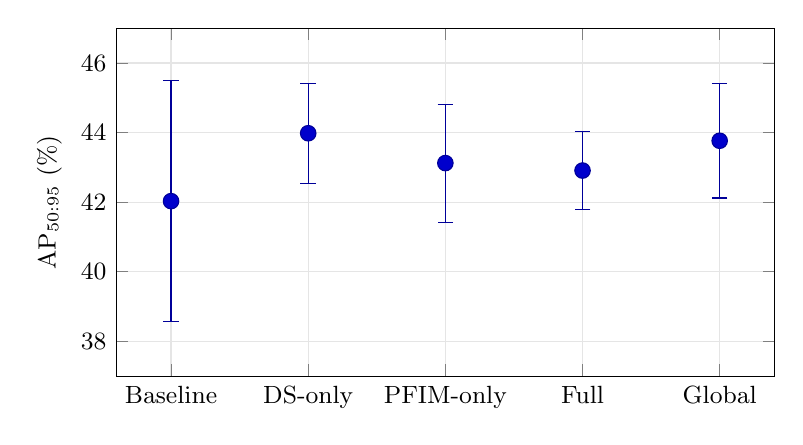
\begin{tikzpicture}
\begin{axis}[width=.82\linewidth,height=6.0cm,ymin=37,ymax=47,
xtick={1,2,3,4,5},xticklabels={Baseline,DS-only,PFIM-only,Full,Global},
ylabel={$\ap_{50:95}$ (\%)},grid=major,grid style={gray!20},
tick label style={font=\small},label style={font=\small}]
\addplot+[only marks,mark=*,mark size=2.8pt,blue!60!black,
error bars/.cd,y dir=both,y explicit] coordinates
{(1,42.0301) +- (0,3.4714) (2,43.9815) +- (0,1.4412)
(3,43.1237) +- (0,1.6957) (4,42.9090) +- (0,1.1289)
(5,43.7656) +- (0,1.6467)};
\end{axis}
\end{tikzpicture}
\caption{SSDD 主指标及跨 seed 离散程度。误差线为样本标准差，不是置信区间；本图不表示统计显著性。}
\label{fig:ssdd}
\end{figure}

PFIM-only 的 recall 均值较基线高约 2.15 pp，但其阈值由各自最优 F1 操作点确定。若论文进一步讨论漏检改善，应增加固定阈值、固定虚警率或完整 PR 曲线比较，而不能直接把这一差值解释为相同操作条件下的目标恢复能力。

\subsection{逐 seed 配对与不确定性}
表\ref{tab:paired}列出同 seed 差值，图\ref{fig:paired}保留全部正负方向。DS-only、PFIM-only 和 Global 各有两次正差、一次负差；Full 只有一次正差。Full 的模型指标标准差虽较小，其相对基线差值的标准差却为 4.57 pp，说明“自身波动小”与“稳定优于基线”并不等价。

\begin{table}[!htbp]\centering\small
\caption{相对同 seed Baseline 的 $\ap_{50:95}$ 配对变化（pp）。}
\label{tab:paired}
\begin{tabular}{lrrrr}
\toprule
变体 & Seed 0 & Seed 1 & Seed 2 & 平均差 $\pm s_d$\\
\midrule
DS-only & $+2.9001$ & $+5.2557$ & $-2.3016$ & $+1.95\pm3.87$\\
PFIM-only & $+2.1274$ & $+3.1558$ & $-2.0026$ & $+1.09\pm2.73$\\
Full / RGSP & $-0.3543$ & $+5.9345$ & $-2.9437$ & $+0.88\pm4.57$\\
Global & $+2.2879$ & $+6.1482$ & $-3.2297$ & $+1.74\pm4.71$\\
\bottomrule
\end{tabular}
\end{table}

\begin{figure}[tbp]\centering
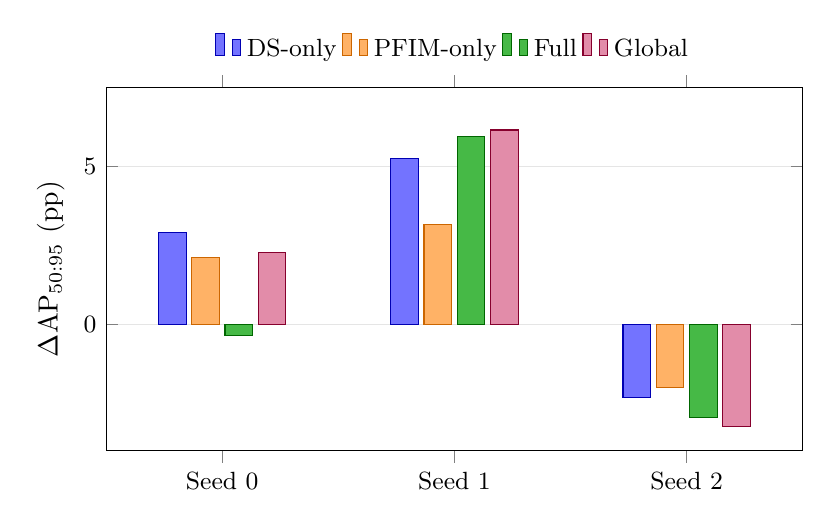
\begin{tikzpicture}
\begin{axis}[width=.86\linewidth,height=6.2cm,ymin=-4.0,ymax=7.5,
ybar,bar width=10pt,xtick={0,1,2},xticklabels={Seed 0,Seed 1,Seed 2},
xmin=-.5,xmax=2.5,ylabel={$\Delta\ap_{50:95}$ (pp)},
legend columns=4,legend style={at={(.5,1.04)},anchor=south,font=\small,draw=none},
ymajorgrids=true,grid style={gray!20},tick label style={font=\small}]
\addplot[fill=blue!55,draw=blue!70!black] coordinates {(0,2.9001)(1,5.2557)(2,-2.3016)};
\addplot[fill=orange!60,draw=orange!80!black] coordinates {(0,2.1274)(1,3.1558)(2,-2.0026)};
\addplot[fill=green!45!gray,draw=green!40!black] coordinates {(0,-.3543)(1,5.9345)(2,-2.9437)};
\addplot[fill=purple!45,draw=purple!70!black] coordinates {(0,2.2879)(1,6.1482)(2,-3.2297)};
\legend{DS-only,PFIM-only,Full,Global}
\end{axis}
\end{tikzpicture}
\caption{同 seed 配对变化。每个 seed 同时对应一个训练/验证划分及一组训练随机性，不能将三个配置当作固定划分下的纯初始化重复。}
\label{fig:paired}
\end{figure}

Seed 2 的 baseline 指标为 45.1215\%，高于另外两次，但仅约高于其三次均值 0.89 个样本标准差，没有依据将其排除为异常值。所有变体在该 seed 相对基线为负是需要保留的观察，而非可以用“划分异常”直接解释的失败。下一轮应分离 split seed 与 training seed，以明确两类变异来源。

\subsection{组合与空间粒度}
Full 相对 DS-only 的逐 seed 差值为 $-3.2544,+0.6788,-0.6421$ pp，平均为 $-1.0726$ pp；Full 相对 Global 为 $-2.6422,-0.2137,+0.2860$ pp，平均为 $-0.8566$ pp。由此，本批记录没有显示完整组合对 DS-only 的优势，也没有显示逐位置 PFIM 对图像级 PFIM 的优势。

这两个观察不能简化为“PFIM 无效”。PFIM-only 的终端指标与 Full 不同，且 Global 仍有逐位置内容和能量变化。更具体的问题是，局部修正、能量条件缩放和重要性控制如何在训练中配合。可能涉及冗余调制、初始化偏移或统计线索的任务适配，但当前终端指标不区分这些解释。由于 Baseline 不是同一替换壳层下的中性单元，上述差值也不等同于严格二因素设计中的统计交互效应。

\subsection{参数量、算子计数与计时}
表\ref{tab:efficiency}保留原包 seed 0 的成本记录。Full 比原始基线少 65,106 个参数，约为 1.09\%；相对 DS-only 增加 2,337 个参数，与 PFIM 的参数推导一致。这说明当前完整替换设计的参数规模没有扩大，但并不证明只添加 RGSP 到不变的原始块也会减少参数。

\begin{table}[!htbp]\centering\small
\caption{seed 0 成本记录。GFLOPs$^\ast$ 未核实自定义 scan 核覆盖；$t_{\rm infer}$ 来自评估器的每图平均推理时间，$1000/t_{\rm infer}$ 不是独立测量的 batch=1 端到端 FPS。}
\label{tab:efficiency}
\begin{tabular}{lrrrr}
\toprule
变体 & 参数量 & GFLOPs$^\ast$ & $t_{\rm infer}$ (ms) & $1000/t_{\rm infer}$\\
\midrule
Baseline & 5,985,547 & 13.61 & 6.616542 & 151.1\\
DS-only & 5,918,104 & 13.12 & 6.000570 & 166.7\\
PFIM-only & 5,920,441 & 13.15 & 6.105006 & 163.8\\
Full / RGSP & 5,920,441 & 13.15 & 6.088878 & 164.2\\
Global & 5,920,441 & 13.15 & 6.129386 & 163.2\\
\bottomrule
\end{tabular}
\end{table}

现有算子计数由项目 profiler 路径生成，未确认对自定义 selective scan 提供完整计数；非零 GFLOPs 并不保证扫描计算已计入。计时还受 batch、同步、预热和预处理/后处理边界影响。因此，本表用于呈现记录及成本量级，不据此宣称 RGSP 获得了已核验的端到端加速。完整效率验证方案见附录\ref{app:plan}。

\subsection{跨任务表现与接入条件}
\paragraph{图像分类。}
表\ref{tab:classification}区分 scratch 与 VMamba 初始化轨道。scratch 下 SAR-ACD 与 SAMPLE 均低于各自基线；VMamba 初始化下，SAR-ACD 无专属预热配置的 Accuracy 较高，额外预热后的记录进一步提高。后者改变了训练预算，不能解释为相同预算下纯模块收益。

\begin{table}[!htbp]\centering\small
\caption{分类探索记录，单 seed，Accuracy / Macro-F1（\%）。各轨道只在行内比较，不跨轨道排名。}
\label{tab:classification}
\begin{tabularx}{\linewidth}{P{2.8cm}P{2.7cm}P{2.7cm}P{1.9cm}Y}
\toprule
轨道/数据集 & Baseline & 历史 P3 & $\Delta$ Accuracy & 条件\\
\midrule
Scratch / SAR-ACD & 94.882 / 94.815 & 89.370 / 89.181 & $-5.512$ & 224，BS64\\
Scratch / SAMPLE & 98.519 / 98.454 & 97.037 / 96.441 & $-1.482$ & real-only 选样\\
VMamba / SAR-ACD & 89.764 / 89.585 & 91.339 / 91.275 & $+1.575$ & 无专属预热\\
VMamba / SAR-ACD & 89.764 / 89.585 & 96.457 / 96.410 & $+6.693$ & P3 额外预热 20e\\
VMamba / SAR-ACD & 89.764 / 89.585 & 96.850 / 96.830 & $+7.086$ & P3 额外预热 50e\\
\bottomrule
\end{tabularx}
\end{table}

\paragraph{语义分割。}
FUSAR-Map 的 mIoU 由 44.297\% 降为 43.561\%；OpenEarthMap-SAR 无专属预热配置由 36.551\% 降为 35.898\%。FUSAR-Map 的 road IoU 从 4.782\% 降到 1.091\%，而 building 和 water 略有增加。这提示应关注细长及低占比类别，而不能仅用整体 OA 评价局部响应修正。该观察没有单独证明是修正项造成了道路退化，因为壳层及接入位置也同时影响结果。

\begin{table}[!htbp]\centering\small
\caption{分割历史记录，单 seed（\%）。“--”表示原汇总未提供该字段，不以零补齐。}
\label{tab:segmentation}
\begin{tabular}{llrrrr}
\toprule
数据集 & 配置 & mIoU & FWIoU & Dice & OA\\
\midrule
FUSAR-Map & Baseline & 44.297 & 65.382 & -- & 77.105\\
FUSAR-Map & P3 & 43.561 & 65.083 & -- & 76.770\\
OpenEarthMap-SAR & Baseline & 36.551 & 36.120 & 50.811 & 52.316\\
OpenEarthMap-SAR & P3，无预热 & 35.898 & 35.220 & 50.163 & 51.764\\
OpenEarthMap-SAR & P3，预热 20e & 35.829 & 36.447 & 49.409 & 52.499\\
OpenEarthMap-SAR & P3，预热 50e & 35.535 & 36.104 & 49.099 & 52.383\\
\bottomrule
\end{tabular}
\end{table}

\paragraph{变化检测。}
在 $m=16$、BS16 记录中，Ottawa 的 F1 从 92.091\% 到 92.249\%，Yellow River 从 88.368\% 到 86.891\%，Farmland 从 23.564\% 到 64.428\%，Sulzberger 从 72.591\% 到 66.180\%。Farmland 的较大改善伴随极低的基线召回（13.887\%），应检查类别不均衡、阈值和基线训练状态，不能直接作为已充分验证的通用机制证据。完整 batch/state 配置及多指标记录见附录\ref{app:cross}.

\paragraph{同名 P3 不保证同一骨干机制。}
当前代码包含三种不同接入路径：检测及 shared \texttt{full\_t} 在 P3/8 内替换后继续计算高层；\texttt{legacy} 路径中名为 P3 的位置实际对应 stride 16；\texttt{vmamba\_tiny} 则先运行完整 encoder，再修改返回的 \texttt{features[1]}，属于输出适配器，不改变已计算的 P4/P5。分类头读取 \texttt{features[1]} 的全局平均池化结果，也不能与最终层分类头混写。图\ref{fig:interfaces}说明两类核心区别。

\begin{figure}[tbp]\centering
\begin{tikzpicture}
\node[font=\small,anchor=east] at (-1.2,1.2) {骨干内部};
\node[box,text width=2.2cm] (a1) at (0.4,1.2) {浅层特征};
\node[box,text width=2.4cm] (a2) at (4.2,1.2) {P3 替换模块};
\node[box,text width=2.4cm] (a3) at (8.2,1.2) {继续计算 P4/P5};
\draw[arrow](a1)--(a2);\draw[arrow](a2)--(a3);
\node[font=\small,anchor=east] at (-1.2,-.7) {输出适配};
\node[box,text width=2.2cm] (b1) at (.4,-.7) {完整 encoder};
\node[box,text width=2.4cm] (b2) at (4.2,-.7) {修改返回特征之一};
\node[box,text width=2.4cm] (b3) at (8.2,-.7) {原 P4/P5 已算完};
\draw[arrow](b1)--(b2);\draw[arrow](b2)--(b3);
\end{tikzpicture}
\caption{接入路径决定方法影响范围。两类路径都可用于任务模型，但不能被当作同一种骨干内部状态更新的统一重复验证。}
\label{fig:interfaces}
\end{figure}
\FloatBarrier

\section{讨论}\label{sec:discussion}
\subsection{可靠性解释与实际控制量}
RGSP 的实际行为是结构条件化状态调制，可靠性是希望通过结构线索刻画的属性，而不是当前已经获得真值监督的输出。验证这层解释需要同时考虑稳定性与任务价值：恒定背景可以稳定但对预测无帮助，目标边缘可以局部变化大但对定位至关重要。仅展示重要性热图与前景重叠，不足以判定控制量刻画了可靠性；仅出现背景高权重，也不足以反向否定它，因为背景上下文可以具有任务价值。

原包保留了历史检查点的六样例 PFIM 审计，其中框内/背景均值比既有约 3.67，也有约 0.45，均值约 1.19、中位数约 0.72。这些例子来自历史验证设置，不是当前三种子矩阵的机制检验。本文保留原图作为来源档案，不用其中挑选的正向例子替代当前模型的定性实验，也不把它称作可靠性真值图。

\subsection{何种证据能够解释方法作用}
现有结果支持对具体实现及配置差异进行描述，但尚未分离局部修正、能量项、重要性输入驱动和步长调制的独立作用。最关键的补充不是增加一组不匹配的外部榜单，而是在同壳层下设置 $\lambda_s=0,q=1,\eta_i=0$ 的中性对照，并增加常数 $q=0.75$、仅局部修正、仅能量项、仅输入驱动和仅步长等控制。该设计可以区分数值缩放、结构替换与结构线索本身的贡献。

如果希望主张该机制可直接增强原始四向 SS2D，还需要在保留原扫描拓扑的实现中单独评估。那属于新方法版本，应重新冻结代码并生成结果，不能将本批单向替换块的成绩改名后作为新版本证据。相同原则也适用于跨任务接口、二维趋势替换和中性初始化等后续改动。

\subsection{跨任务结论及研究局限}
当前实验最有辨识度的观察是：DS-only 的检测均值较高，但完整组合不优于 DS-only，图像级重要性也未被逐位置预测超越。跨任务结果呈现不同方向，说明泛化评价需要同时控制任务头、输入、初始化、训练预算和真实接入位置。任务无关的模块接口为迁移提供了技术可能性，但不自动构成跨任务收益。

本研究的局限集中在四方面：第一，检测主证据来自一个数据集和三组联合变化的随机配置；第二，原块与替换块存在扫描及壳层差异；第三，部分训练原始产物尚未随稿归档，调度和历史选模版本需闭合；第四，自定义算子成本和独立可靠性诊断尚未完整测量。附录\ref{app:plan}将这些限制转化为可执行、可验收的实验设计，而非用推测性数字填补。

\section{结论}
本文提出 RGSP，以局部趋势和二维邻域变化作为结构线索，将可学习局部残差修正与空间重要性控制引入 Mamba 的输入驱动和离散化步长。精确递推分析表明，这两类控制分别影响当前驱动与状态演化，不能被简化为三个独立的保留/写入门。SSDD 记录中，完整 RGSP 的 $\ap_{50:95}$ 均值较基线高 0.88 pp，但未超过 DS-only；逐位置重要性未超过图像级对照。分类、分割和变化检测进一步展示了适用条件的差异。由此，本文将局部结构线索如何参与选择性递推明确为一个可复现、可拆解验证的研究问题；其可靠性解释和更广泛收益仍需由同结构控制及统一跨任务验证建立。
\FloatBarrier
\appendix
\section{符号、实现与变体补充}\label{app:implementation}
\begin{table}[H]\centering\small
\caption{核心张量、参数与当前检测路径。}
\begin{tabularx}{\linewidth}{P{2.7cm}P{3.5cm}Y}
\toprule
符号 & 形状/取值 & 含义\\
\midrule
$X,\bar X,\widetilde X$ & $b\times L\times d$ & 归一化输入、序列趋势、修正特征\\
$S,V$ & $b\times L\times d$；$b\times L\times2d$ & 二维局部标准差及拼接描述子\\
$I$ & $b\times L\times1$ & 每位置一个控制标量，跨通道广播\\
$u,z,\Delta$ & $b\times L\times d$ & 内容、输出门、离散化步长\\
$B_t,C_t$ & $b\times m$ & 当前位置的状态写入/读出向量\\
$A,h_t$ & $d\times m$；$b\times d\times m$ & 负对角生成元参数、隐藏状态\\
$D$ & $d$ & 修正特征旁路系数\\
$d,m$ & 当前 P3 为 64、16 & 通道数与状态维数\\
$\lambda_s,\alpha,\beta_i,\rho_i,\eta_i$ & 初始 $0.5,0.5,1,1,0.1$ & 块级可学习标量，符号无约束\\
$g_{\min},s_n,\epsilon$ & $0.5,0.1,10^{-5}$ & 固定缩放与数值稳定常数\\
\bottomrule
\end{tabularx}
\end{table}

实现顺序为：归一化序列 $\rightarrow$ 可学习趋势和局部修正 $\rightarrow$ 二维统计及 PFIM $\rightarrow$ 投影生成 $u,z,B,C$ $\rightarrow$ 构造 $q,\Delta$ $\rightarrow$ selective scan $\rightarrow$ 加 $D\widetilde X$ $\rightarrow$ $\SiLU(z)$ 门控与输出投影。实际顺序决定某个改动会影响哪些分支，不能把图上的所有控制量都解释为同一注意力操作。

关闭二维统计的历史开关会改用一维局部标准差，而非删除标准差分支。因此，这一变体应命名为“2D 对 1D 统计”，不能在消融中标为“无统计”。新增真正的无统计对照需要固定替代输入并重新运行。

\section{SSDD 逐 run 结果}\label{app:individual}
\begin{table}[H]\centering\small
\caption{SSDD 测试记录（\%）。每行对应原包一条记录，不将四舍五入后的显示数用于二次计算。}
\begin{tabular}{lrrrrrr}
\toprule
变体 & Seed & $\ap_{50}$ & $\ap_{75}$ & $\ap_{50:95}$ & P & R\\
\midrule
Baseline & 0 & 87.1822 & 35.6859 & 42.6943 & 89.2285 & 80.4029\\
Baseline & 1 & 83.6934 & 28.1695 & 38.2746 & 87.8971 & 77.2894\\
Baseline & 2 & 88.6714 & 38.2830 & 45.1215 & 91.5192 & 80.0366\\
DS-only & 0 & 87.1986 & 41.9141 & 45.5944 & 90.9989 & 79.4872\\
DS-only & 1 & 87.3584 & 35.8419 & 43.5303 & 89.3584 & 79.9723\\
DS-only & 2 & 85.5283 & 34.9699 & 42.8199 & 89.3093 & 79.5616\\
PFIM-only & 0 & 90.0920 & 38.1567 & 44.8217 & 90.6961 & 83.9133\\
PFIM-only & 1 & 87.3274 & 30.4719 & 41.4304 & 88.6802 & 80.4029\\
PFIM-only & 2 & 87.2713 & 35.8535 & 43.1189 & 91.0193 & 79.8535\\
Full & 0 & 88.0882 & 30.7187 & 42.3400 & 93.2318 & 80.7692\\
Full & 1 & 87.8664 & 36.8629 & 44.2091 & 92.2132 & 78.7546\\
Full & 2 & 87.9535 & 34.7167 & 42.1778 & 90.2943 & 80.0366\\
Global & 0 & 86.8336 & 40.0310 & 44.9822 & 91.9194 & 78.0220\\
Global & 1 & 86.7447 & 38.0432 & 44.4228 & 90.8392 & 77.8388\\
Global & 2 & 85.6446 & 32.5236 & 41.8918 & 92.5226 & 79.4872\\
\bottomrule
\end{tabular}
\end{table}
随稿 CSV 还保留逐 run 权重 SHA-256。哈希标识权重内容，但不能单独证明数据划分、训练参数和评估访问过程；复现需要同时绑定这些记录。原始汇总与本次复算分别保存，未改动输入数据。

\section{跨任务协议与完整记录}\label{app:cross}
\subsection{分类数据与接口}
本地 SAR-ACD 集合记录为 2,522 张、5 类；不与其他文献中的六类或不同样本量版本混合。当前修订未将该本地集合与唯一首发文献及发布版本完成绑定，故不以近似同名论文代替数据来源。SAMPLE 使用项目筛选的 real-only 子集；其来源论文\cite{sample2019}不自动赋予本地子集与原论文协议相同的资格。

scratch 记录使用输入 224、batch 64、最多 200 epochs、seed 0。VMamba 初始化轨道还包括模块预热 20/50 epochs，预热后再进行正式训练；其总预算与没有这段日程的基线不同。当前分类头使用第二个返回特征的全局平均池化、归一化与线性分类，而非默认取最终骨干层。此接口使新增模块参与分类，但也改变了与常规最终层分类协议的对应关系。

\subsection{变化检测}
每个数据集包含一个配准图像对，记录尺寸分别为 Ottawa $350\times290$、Yellow River $289\times257$、Farmland $291\times306$、Sulzberger $256\times256$。历史说明采用 $48\times48$ 裁块并缩放到训练输入 192，以空间区域构造训练、验证和测试部分。空间不重叠与感受野不泄漏并非同一条件，最终确认需检查源坐标、裁块重叠和边界缓冲区，不能仅根据样本数认定已完成空间隔离审计。

$m=16$ 记录为 scratch、150 epochs、AdamW/cosine、seed 0。两时相共享骨干，对相应层特征取绝对差后送入任务解码器；未来同任务对照应保持该头及损失不变。表\ref{tab:cd16}列出历史各 batch 结果。

\begin{table}[H]\centering\small
\caption{变化检测历史结果，$m=16$、seed 0（\%）。不同 batch 为不同配置，不作独立重复统计。}
\label{tab:cd16}
\setlength{\tabcolsep}{4pt}
\begin{tabular}{llrrrrrr}
\toprule
数据集 & 配置 & BS & P & R & F1 & IoU & OA\\
\midrule
Ottawa & Baseline & 16 & 90.259 & 94.000 & 92.091 & 85.342 & 98.351\\
Ottawa & P3 & 16 & 88.777 & 96.003 & 92.249 & 85.612 & 98.352\\
Ottawa & Baseline & 96 & 87.953 & 95.147 & 91.409 & 84.177 & 98.173\\
Ottawa & P3 & 96 & 89.841 & 94.346 & 92.039 & 85.251 & 98.333\\
Yellow River & Baseline & 16 & 91.205 & 85.702 & 88.368 & 79.160 & 97.817\\
Yellow River & P3 & 16 & 91.422 & 82.787 & 86.891 & 76.820 & 97.584\\
Yellow River & Baseline & 96 & 89.377 & 78.320 & 83.484 & 71.650 & 97.002\\
Yellow River & P3 & 96 & 91.218 & 71.146 & 79.941 & 66.585 & 96.546\\
Farmland & Baseline & 16 & 77.704 & 13.887 & 23.564 & 13.355 & 92.778\\
Farmland & P3 & 16 & 93.259 & 49.213 & 64.428 & 47.523 & 95.644\\
Farmland & Baseline & 96 & 80.623 & 12.532 & 21.692 & 12.165 & 92.747\\
Farmland & P3 & 96 & 91.747 & 50.719 & 65.325 & 48.506 & 95.684\\
Sulzberger & Baseline & 16 & 75.922 & 69.540 & 72.591 & 56.974 & 90.461\\
Sulzberger & P3 & 16 & 51.656 & 92.066 & 66.180 & 49.454 & 82.908\\
\bottomrule
\end{tabular}
\end{table}

\begin{table}[H]\centering\small
\caption{后续 $m=32$、BS16、seed 0 配置（F1，\%）。与表\ref{tab:cd16}分开报告。}
\label{tab:cd32}
\begin{tabular}{lrrr}
\toprule
数据集 & Baseline & P3 & $\Delta$ F1 (pp)\\
\midrule
Ottawa & 92.758 & 92.110 & $-0.648$\\
Yellow River & 88.079 & 87.689 & $-0.390$\\
Farmland & 26.050 & 73.104 & $+47.054$\\
\bottomrule
\end{tabular}
\end{table}
原包给出该 $m=32$ P3 配置的参数量 2.144M、GFLOPs 1.137；由于扫描算子覆盖及计时协议未闭合，此处不以其建立跨模型效率排名。

\subsection{分割}
FUSAR-Map 采用四类 UPerNet-lite 诊断设置，输入 256、batch 10、FP32、最多 150 epochs，按验证 mIoU 选模。记录的训练/验证/测试块数为 17,560/4,390/1,280；源场景与裁块清单仍需以原始 manifest 绑定。四类 IoU 见表\ref{tab:classiou}。

\begin{table}[H]\centering\small
\caption{FUSAR-Map 类别 IoU（\%），保留低占比道路类别的退化。}
\label{tab:classiou}
\begin{tabular}{lrrrr}
\toprule
配置 & Building & Vegetation & Water & Road\\
\midrule
Baseline & 14.280 & 71.493 & 86.634 & 4.782\\
P3 & 15.231 & 71.075 & 86.846 & 1.091\\
\bottomrule
\end{tabular}
\end{table}

OpenEarthMap-SAR 的历史设置使用 SAR-only 输入、VMamba-Tiny ImageNet 初始化、P3-$m=16$、训练输入 512、测试输入 1024、seed 0、150 epochs。记录描述物理 batch 32 加梯度累积 2；实际有效 batch 应由对应 run 的配置确认。Baseline、无预热 P3、预热 20e 和 50e 的 mPA 分别为 58.090、54.914、49.055 和 49.563\%。预热配置只在对应轨道内分析，不以 OA 单项微小改善替代主 mIoU 结论。
\FloatBarrier

\section{历史检测与公开作者报告}\label{app:history}
\subsection{单种子记录}
\begin{table}[H]\centering\small
\caption{历史检测 $\ap_{50:95}$（\%）。不同设置分别报告，不计算跨行总体平均。}
\label{tab:history}
\begin{tabularx}{\linewidth}{P{2.2cm}P{4.0cm}rrrY}
\toprule
数据集 & 设置 & Baseline & P3 & 差值 (pp) & 范围\\
\midrule
SSDD & scratch，BS16，150e & 35.239 & 42.991 & $+7.752$ & 单 seed\\
SSDD & scratch，BS32，150e & 45.683 & 42.486 & $-3.197$ & 独立批次\\
SADD & scratch，BS32，200e & 55.018 & 54.597 & $-0.421$ & 单 seed\\
AIR-SARShip-2.0 & 源图划分后切片，BS32，200e & 17.375 & 19.291 & $+1.916$ & scratch\\
OGSOD-1.0 & 输入1024，300e，全局BS64 & 42.302 & 43.602 & $+1.300$ & 单次匹配\\
\bottomrule
\end{tabularx}
\end{table}
这些记录独立于 SSDD 当前五变体矩阵。SSDD 两个 batch 配置方向相反，说明有必要检查训练和数据条件，但不能仅凭两次结果给出 batch 效应的因果解释。OGSOD 为历史探索，不自动重新纳入当前主验证矩阵。

\subsection{协议不匹配及失败记录}
\begin{table}[H]\centering\small
\caption{不能作为当前公平主比较的历史结果，$\ap_{50:95}$（\%）。}
\begin{tabularx}{\linewidth}{P{3.35cm}P{2.7cm}Y}
\toprule
记录 & 数值 & 不可直接比较的原因\\
\midrule
SSDD ex27 TEST & Baseline 70.348；P3 71.445 & 历史检查点与部分迁移初始化；VAL 74.022 不是 TEST\\
SSDD 部分迁移 300e & P3 72.261 & 无匹配基线，不能计算净增益\\
SADD 部分迁移 300e & P3 72.113 & 无匹配基线；不能并入 scratch\\
SRSDD-v1.0 HBB & P3 22.147 & 水平框转换与公开旋转框任务不同\\
SAR-ShipDataset & Baseline 49.568；P3 57.818 & baseline 训练 batch 中途变化，不是严格配对\\
SAR-AIRcraft patch TEST & Baseline 54.513；P3 55.552 & 优化器、batch、轮数不一致；patch 与原图口径不同\\
SAR-AIRcraft 失败运行 & 不报告最终 TEST & 非有限 loss 中止；中间验证 AP 不能作为测试成绩\\
\bottomrule
\end{tabularx}
\end{table}

SAR-AIRcraft 历史 patch 数据使用 512 像素重叠裁片，训练/验证/测试分别记录为 13,976/1,923/2,989 个 patch，模型输入 1024。Baseline 为 SGD、BS16、约137 epochs；P3 为 AdamW、全局 BS48、300 epochs。其 patch VAL 的 $\ap_{50}$ 为 87.751/88.825\%，$\ap_{50:95}$ 为 69.904/70.513\%；patch TEST 的 $\ap_{50}$ 为 70.402/70.822\%。这些差异不能被解释为单个模块效应。

SAR-ShipDataset 历史本地划分记录为 31,783/3,972/3,974，模型输入512，$\ap_{50}$ 为94.616/94.844\%。这些本地集合数不等同于正式数据集论文的整体数据规模，且 baseline batch 曾从256改为128。另一个 SAR-AIRcraft FP32 运行在 epoch15、batch166 出现非有限损失，epoch14 验证 $\ap_{50:95}=53.902\%$ 仅是中间过程值；没有将其填入最终结果表。

\subsection{公开结果只作版本明确的文献背景}
表\ref{tab:author}仅列 MaDiNet 预印本 v1 自身报告的三项主指标\cite{madinet2024v1}。其正式期刊版本作为相关工作单独引用\cite{madinet2025}，但不将两个版本的作者、实现和数字互相替换。本文没有对这些配置执行同协议复现，也不将本地 scratch 结果放在同一排行榜中。

\begin{table}[H]\centering\small
\caption{Author-reported：MaDiNet 预印本 v1 的 $\ap_{50}$（\%），来源为其对应数据集主结果表。与本地实验未做协议匹配。}
\label{tab:author}
\begin{tabular}{lrc}
\toprule
数据集 & MaDiNet & 本文同协议复现\\
\midrule
SSDD & 99.0 & 未完成\\
SAR-ShipDataset & 97.5 & 未完成\\
SAR-AIRcraft-1.0 & 90.5 & 未完成\\
\bottomrule
\end{tabular}
\end{table}
后续外部比较应选择与目标资源预算匹配的公开检测器，并明确引用其原论文或官方实现。若采用文献中的二手对比数字，应标注转引来源，不能让读者误认为由本文重新运行。
\FloatBarrier

\section{待完成的确认实验设计}\label{app:plan}
本节是后续实验方案，不是新增实验结果。其目的是把方法假设转化为明确控制和验收条件；所有运行均需另行冻结代码、数据与资源配置。

\subsection{优先级 P0：同结构对照与协议闭合}
首先回收15个 run 的原始划分、训练参数、源码快照、日志和测试输出，核定学习率调度及 checkpoint 选择规则。随后在\emph{同一替换壳层}内建立中性基准：$\lambda_s=0,q_t\equiv1,\eta_i=0$，其余归一化、投影、MLP、状态维数和输出路径保持一致。新增这些对照是新实验，不用已有 Baseline 冒充中性单元。

\begin{table}[H]\centering\small
\caption{建议的同壳层机制控制矩阵，全部为 Planned。}
\label{tab:planned-controls}
\begin{tabularx}{\linewidth}{P{3.0cm}P{4.6cm}Y}
\toprule
对照 & 唯一目标改动 & 回答的问题\\
\midrule
中性替换壳层 & $\lambda_s=0,q=1,\eta_i=0$ & 壳层变化的整体影响\\
常数驱动 & 相对中性设 $q=0.75$ & 常数缩放能否解释部分差异\\
仅局部修正 & 启用 $\lambda_s$ 与趋势；保持 $q=1,\eta_i=0$ & 修正项的增量作用\\
仅能量条件项 & 在同壳层内启用 $E$ 条件缩放 & 能量项与常数缩放的区别\\
PFIM 输入驱动 & 仅让 $I$ 影响 $q$ & 空间控制对当前写入的作用\\
PFIM 步长 & 保持 $q=1$，仅让 $I$ 影响 $\Delta$ & 离散化调制的作用\\
驱动与步长联合 & 同时启用两类位置 & 两个位置的组合关系\\
全局/局部/常数 $I$ & 其余分支、容量和预算一致 & 空间粒度的净影响\\
\bottomrule
\end{tabularx}
\end{table}

若研究问题要求增强原始 SS2D，则在保留其四方向扫描、归一化、投影和前馈分支的前提下只改调制路径；该四向实现与本稿单向实现分版本报告。二维趋势对一维趋势的比较也应作为独立因素，特别检查行边界响应，避免把统计窗口、拓扑和容量同时变化后仍称单因素消融。

\subsection{优先级 P1：可靠性线索和注入位置}
可靠性评价需先定义与 $I$ 独立的代理目标。例如，在预先确定的标签保持扰动下，以配准后的特征或预测一致性衡量稳定性，同时检查目标定位或分类相关性，避免把稳定但无任务价值的背景当作可靠性全部含义。扰动范围应保证标签有效；无干净配对真值时，不把特征差解释为物理去斑质量。

对控制量的干预包括常数替代、空间置换和跨样本交换，并在保持内容流固定时观察变化。冻结模型上的干预可能造成分布外输入，需结合训练期匹配对照；不能把任何置换后的降分都当作可靠性机理的证明。还应对比同容量输入特征重加权、扫描输出重加权与内部步长调制，以定位收益来源。

可视化应使用预先固定的样例集合，包含近岸/离岸、弱小目标、密集区域、强散射背景和失败样例。展示原输入、预测、误差、$I$、$q$ 与 $\Delta$ 的统计，而非只画视觉上有利的热图。尺度与背景分组规则在观察测试结果前冻结；报告样本数及分组不确定性，不根据结果修改分组阈值。

\subsection{优先级 P1：检测主验证与四任务迁移}
检测主验证按 SSDD、SAR-ShipDataset、SAR-AIRcraft-1.0 分别冻结原图或 patch 协议、初始化和评价器；主对照为相同基线与加入 RGSP 后的对应模型。机制筛选在训练/验证部分完成，再使用独立确认评估，不能不断利用已看过的测试成绩选择最终模块。

随机性建议分两层组织：先固定一个数据划分进行预先约定数量的训练重复，再在额外固定划分上检查敏感性，分别报告两类方差。重复数与停止条件应在实验前确定，不能“跑到显著为止”。每个 run 保留失败及原因是否已知，不仅保留成功或最优 seed。

\begin{table}[H]\centering\small
\caption{跨任务受控验证要求，全部为 Planned。跨任务可使用不同头，但同任务的一对模型必须保持头、损失和预算一致。}
\begin{tabularx}{\linewidth}{P{2.1cm}P{3.7cm}YY}
\toprule
任务 & 必须固定的接口 & 主要指标 & 特别检查\\
\midrule
检测 & 同一骨干位置、颈部、检测头 & $\ap_{50:95}$、$\ap_{50}$、P/R & HBB/OBB、原图/patch、NMS与选模\\
分类 & 同一骨干输出层、池化及分类头 & Accuracy、Macro-F1 & 同类集合、样本源、无单侧预热\\
分割 & 同一编码器插入位置及解码器 & mIoU、类别IoU & 源场景隔离、细长/少数类\\
变化检测 & 同一双时相共享骨干及差分头 & F1、IoU & 空间缓冲、阈值、类别不平衡\\
\bottomrule
\end{tabularx}
\end{table}

若某任务只能使用输出适配器，应将其标为适配器实验，不能并入“骨干内部更新”的统一机制结论。外部公开方法用于评价竞争力，内部同框架对照用于分析方法增量；两类实验各自回答不同问题。

\subsection{优先级 P2：效率、复现与报告}
完整模型效率在相同硬件、输入、精度和 batch 下比较，分别报告 batch=1 延迟与较大 batch 吞吐。固定预热次数、测量重复次数和同步方式，给出延迟分布而不仅是一次均值；明确是否包含数据搬运、预处理和 NMS。算子计数必须说明 selective scan 的处理规则，同时报告参数量和峰值显存。

最终结果按实测、作者报告、历史记录和待完成四类分开。若新的严格对照仍显示 Full 不优于简化版本，应以确认后的有效机制组织论文，不以删除负结果或改换指标维持原先叙事。研究结论随证据更新，方法名称也应与可靠性验证的完成程度一致。

\section{证据归档与版本说明}\label{app:provenance}
本修订以用户提供的 Overleaf 源包为基础，保留其原始逐 run CSV、汇总 CSV及历史图件。所有正文图为本稿内嵌矢量图或由已有数值绘制的统计图，没有新增训练、推理或模拟结果。主文的数值复算使用原始精度和样本标准差。

\begin{table}[H]\centering\small
\caption{复现所需材料及当前包的覆盖边界。}
\begin{tabularx}{\linewidth}{P{3.8cm}YY}
\toprule
材料 & 当前覆盖 & 最终确认要求\\
\midrule
逐 run 指标与权重哈希 & 原包已提供，修订保留 & 与原始评估 JSON 和权重逐项关联\\
训练/验证/测试清单 & 有文档描述，完整原始链未随包附齐 & 固定文件清单、源场景ID与内容哈希\\
训练参数与学习率日程 & 有协议及计划，存在差异 & 每个 run 的真实参数与学习率曲线\\
源码与选模版本 & 已静态核对当前实现 & 保存实际 run 使用的源码快照和修改差异\\
扫描后端与成本 & 有实现和历史计数 & 后端标识、算子覆盖及测量配置\\
跨任务数据来源 & 历史同名数据及部分论文来源 & 明确发布版本、子集、许可及划分对应\\
参考文献 & 每项按论文/DOI/版本定位 & 文中论述与对应来源逐条匹配\\
\bottomrule
\end{tabularx}
\end{table}

随包的文献对照表区分“书目信息已核对”和“具体方法描述已由原文支持”。某篇论文被正确收录并不意味着其中所有实验结论都可迁移到本文。原始历史协议文件作为来源保存，不再作为没有冲突的现行实验规范；修订澄清以本稿及对应说明为准。
\FloatBarrier

\begin{thebibliography}{99}
\small
\bibitem{ssdd2021}
T. Zhang, X. Zhang, J. Li, et al.
SAR Ship Detection Dataset (SSDD): Official Release and Comprehensive Data Analysis.
\emph{Remote Sensing}, 13(18):3690, 2021.
\url{https://doi.org/10.3390/rs13183690}.

\bibitem{saraircraft2023}
王智睿，康玉卓，曾璇，汪越雷，张汀，孙显.
SAR-AIRcraft-1.0：高分辨率SAR飞机检测识别数据集.
\emph{雷达学报}, 12(4):906--922, 2023.
\url{https://doi.org/10.12000/JR23043}.

\bibitem{resnet2015}
K. He, X. Zhang, S. Ren, and J. Sun.
Deep Residual Learning for Image Recognition.
\emph{IEEE Conference on Computer Vision and Pattern Recognition (CVPR)},
pp. 770--778, 2016.
\url{https://doi.org/10.1109/CVPR.2016.90}.

\bibitem{vit2020}
A. Dosovitskiy, L. Beyer, A. Kolesnikov, et al.
An Image is Worth 16x16 Words: Transformers for Image Recognition at Scale.
\emph{International Conference on Learning Representations (ICLR)}, 2021.
\url{https://arxiv.org/abs/2010.11929}.

\bibitem{mamba2023}
A. Gu and T. Dao.
Mamba: Linear-Time Sequence Modeling with Selective State Spaces.
arXiv:2312.00752, 2023.
\url{https://arxiv.org/abs/2312.00752}.

\bibitem{vim2024}
L. Zhu, B. Liao, Q. Zhang, X. Wang, W. Liu, and X. Wang.
Vision Mamba: Efficient Visual Representation Learning with Bidirectional State Space Model.
\emph{International Conference on Machine Learning (ICML)}, 2024.
\url{https://arxiv.org/abs/2401.09417}.

\bibitem{vmamba2024}
Y. Liu, Y. Tian, Y. Zhao, et al.
VMamba: Visual State Space Model.
\emph{Advances in Neural Information Processing Systems (NeurIPS)}, 2024.
\url{https://arxiv.org/abs/2401.10166}.

\bibitem{mambayolo2024}
Z. Wang, C. Li, H. Xu, X. Zhu, and H. Li.
Mamba YOLO: A Simple Baseline for Object Detection with State Space Model.
arXiv:2406.05835, 2024.
\url{https://arxiv.org/abs/2406.05835}.

\bibitem{rsmamba2024}
S. Zhao, H. Chen, X. Zhang, P. Xiao, L. Bai, and W. Ouyang.
RS-Mamba for Large Remote Sensing Image Dense Prediction.
\emph{IEEE Transactions on Geoscience and Remote Sensing}, 62:1--14, 2024.
\url{https://doi.org/10.1109/TGRS.2024.3425540}.

\bibitem{rstmtmamba2025}
Y. Shen, L. Xiao, J. Chen, Q. Du, and Q. Ye.
Learning Cross-Task Features With Mamba for Remote Sensing Image Multitask Prediction.
\emph{IEEE Transactions on Geoscience and Remote Sensing}, 63:1--16, 2025.
\url{https://doi.org/10.1109/TGRS.2025.3540573}.

\bibitem{madinet2025}
J. Zhou, Y. Liu, B. Peng, L. Liu, and X. Li.
MaDiNet: Mamba Diffusion Network for SAR Target Detection.
\emph{IEEE Transactions on Circuits and Systems for Video Technology},
35(11):10787--10800, 2025.
\url{https://doi.org/10.1109/TCSVT.2025.3574657}.

\bibitem{lee1980}
J.-S. Lee.
Digital Image Enhancement and Noise Filtering by Use of Local Statistics.
\emph{IEEE Transactions on Pattern Analysis and Machine Intelligence},
PAMI-2(2):165--168, 1980.
\url{https://doi.org/10.1109/TPAMI.1980.4766994}.

\bibitem{specklefree2021}
S.-W. Chen, X.-C. Cui, X.-S. Wang, and S.-P. Xiao.
Speckle-Free SAR Image Ship Detection.
\emph{IEEE Transactions on Image Processing}, 30:5969--5983, 2021.
\url{https://doi.org/10.1109/TIP.2021.3089936}.

\bibitem{rssnet2026}
M. Huang, Y. Yang, and Q. Sun.
RSS-Net: A Mamba-Based Network for SAR Image Denoizing.
\emph{IEEE Journal of Selected Topics in Applied Earth Observations and Remote Sensing},
19:3539--3551, 2026.
\url{https://doi.org/10.1109/JSTARS.2025.3647971}.

\bibitem{mambadip2026}
Chinchu A, A. A. Bini, and P. Jidesh.
MambaDIP: Mamba-Based Deep Image Prior Framework for Despeckling and Enhancement of SAR Images.
\emph{IEEE Journal of Selected Topics in Applied Earth Observations and Remote Sensing},
19:21255--21271, 2026.
\url{https://doi.org/10.1109/JSTARS.2026.3702550}.

\bibitem{madinet2024v1}
J. Zhou, C. Xiao, B. Peng, T. Liu, Z. Liu, Y. Liu, and L. Liu.
MaDiNet: Mamba Diffusion Network for SAR Target Detection.
arXiv:2411.07500v1, 2024.
\url{https://arxiv.org/abs/2411.07500v1}.

\bibitem{mcmn2026}
G. Gao, C. Li, X. Zhang, B. Yao, and Z. Chen.
Mamba-CNN hybrid Multi-scale ship detection Network driven by a Dual-perception feature of Doppler and Scattering.
\emph{ISPRS Journal of Photogrammetry and Remote Sensing}, 232:656--674, 2026.
\url{https://doi.org/10.1016/j.isprsjprs.2026.01.004}.

\bibitem{cbam2018}
S. Woo, J. Park, J.-Y. Lee, and I. S. Kweon.
CBAM: Convolutional Block Attention Module.
\emph{European Conference on Computer Vision (ECCV)}, 2018.
\url{https://arxiv.org/abs/1807.06521}.

\bibitem{sarship2019}
Y. Wang, C. Wang, H. Zhang, Y. Dong, and S. Wei.
A SAR Dataset of Ship Detection for Deep Learning under Complex Backgrounds.
\emph{Remote Sensing}, 11(7):765, 2019.
\url{https://doi.org/10.3390/rs11070765}.

\bibitem{sample2019}
B. Lewis, T. Scarnati, E. Sudkamp, J. Nehrbass, S. Rosencrantz, and E. Zelnio.
A SAR dataset for ATR Development: the Synthetic and Measured Paired Labeled Experiment (SAMPLE).
In \emph{Algorithms for Synthetic Aperture Radar Imagery XXVI}, SPIE, 2019.
\url{https://doi.org/10.1117/12.2523460}.

\bibitem{fusar2021}
X. Shi, S. Fu, J. Chen, F. Wang, and F. Xu.
Object-Level Semantic Segmentation on the High-Resolution Gaofen-3 FUSAR-Map Dataset.
\emph{IEEE Journal of Selected Topics in Applied Earth Observations and Remote Sensing},
14:3107--3119, 2021.
\url{https://doi.org/10.1109/JSTARS.2021.3063797}.

\bibitem{oemsar2025}
J. Xia, H. Chen, C. Broni-Bediako, Y. Wei, J. Song, and N. Yokoya.
OpenEarthMap-SAR: A benchmark synthetic aperture radar dataset for global high-resolution land cover mapping [Software and Data Sets].
\emph{IEEE Geoscience and Remote Sensing Magazine}, 13(4):476--487, 2025.
\url{https://doi.org/10.1109/MGRS.2025.3599512}.

\bibitem{adamw2017}
I. Loshchilov and F. Hutter.
Decoupled Weight Decay Regularization.
\emph{International Conference on Learning Representations (ICLR)}, 2019.
\url{https://arxiv.org/abs/1711.05101}.

\bibitem{coco2014}
T.-Y. Lin, M. Maire, S. Belongie, et al.
Microsoft COCO: Common Objects in Context.
\emph{European Conference on Computer Vision (ECCV)}, pp. 740--755, 2014.
\url{https://doi.org/10.1007/978-3-319-10602-1_48}.
\end{thebibliography}
\end{document}
